\documentclass[titlepage]{article}
\usepackage[left=2.54cm,top=2.54cm,right=2.54cm,nohead]{geometry}
\usepackage{graphicx}
\setlength{\parskip}{2mm}
\title{User Manual for [Product]}
\author{Yubin Kim, Daniel Burstyn, Gobaan Raveendran, Nathaniel Flath}
\begin{document}
\maketitle
\newpage
\tableofcontents
\newpage

\section{Introduction}
This may be useful for code: \verb!verbatim text!

This is how you embed graphics:

\begin{center}
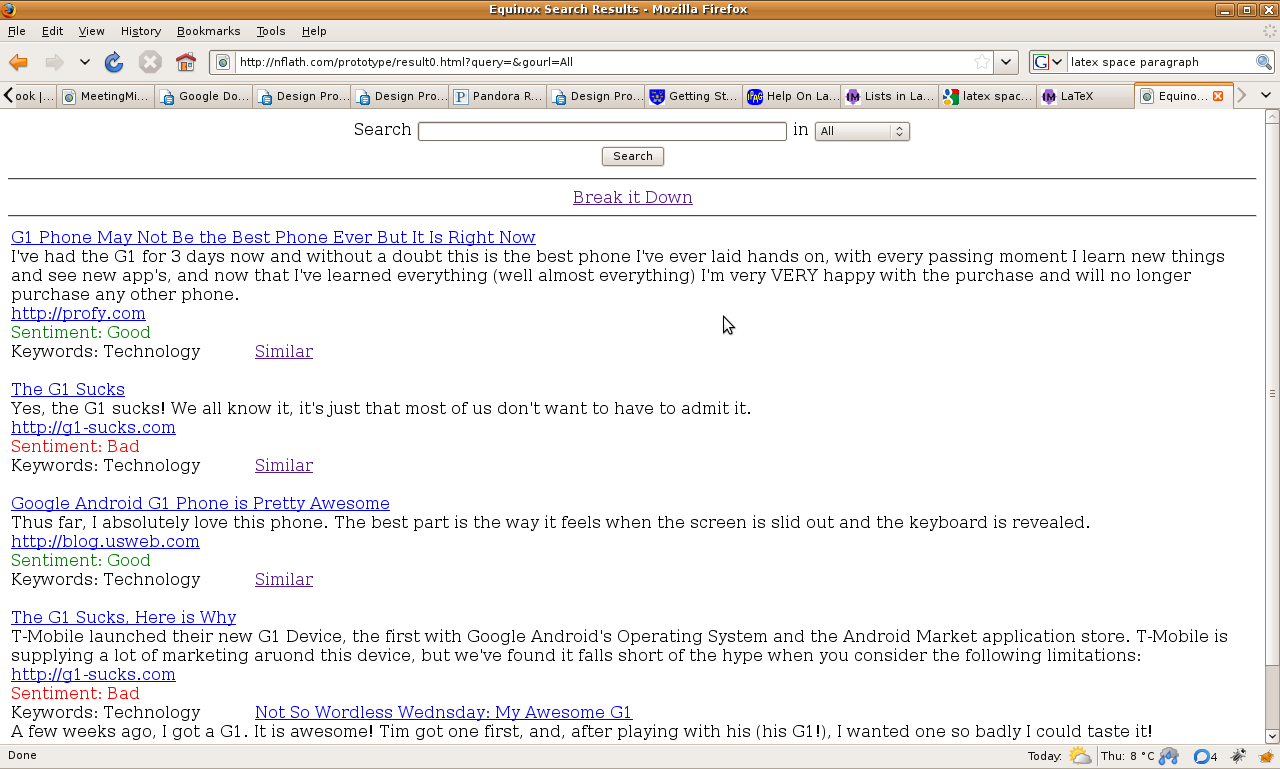
\includegraphics[width=15cm]{screenshot.png}
\end{center}

\subsection{Outline}

\subsection{Product Overview and Motivation}
\begin{itemize}
\setlength{\itemsep}{-1mm}
\item aka, rationale
\item rationale 1: for our data access use case; gathering/cleaning data takes
a long time etc. i
\item rationale 2: for sentiment search use case; describe a sample run using
Google, and using [Product]
\item quick description of product (emphasize product is two-fold; it provides
a large collected/clean data for additional research, and it does sentiment
search)
\end{itemize}

\section{Website Features}
\begin{itemize}
\setlength{\itemsep}{-1mm}
\item describe search features as outlined
http://nflath.com/wiki/index.php/MeetingMinutes
\item mention help page and how to get there
\item provide screen shots (we will, of course, substitute these later after
sprucing up webpage)
\end{itemize}

\subsection{Help Mode}
Users can get help with our product by clicking a `help' link on any of our
pages.  This link redirects to help on the page they just came from; if
clicked on our main page, it will explain the purpose of our product and how
to use it.  This `main' help page will also be accessible from all other help
pages.  If `help' is clicked on a results page, the opened page will also
explain how to interpret the results presented.

    TODO: screenshot

The above screenshot shows the main help page.  As described previously, it
has basic information about our product and how to use it.  It additionally
links to this document, or an updated user manual.  The help navigation tree
is on the left, allowing the user to easily access help on any feature they
desire.

    TODO: mock-up screenshots of help page

The above screenshot shows a sample help web page for an analysis page.  As
you can see, each feature on the page has an explanation---the visualization
explains how the data was broken down, each column of data has an explanation
describing it, etc.  This page describes to the user precisely what they are
looking at and what they can do in order to clear any confusion they may
have.

\section{Advanced Features}
\begin{itemize}
\item insert blurb here about the fact that we provide APIs and what situation
they can be used
\end{itemize}

\subsection{Data Access API}
Should contain examples. This is some
Lorem ipsum dolor sit amet, consectetur adipiscing elit. Integer sit amet nunc
sapien. Aenean eu felis leo, eget rhoncus risus. In tempus nunc ac ipsum
sagittis fringilla. Morbi volutpat, diam quis condimentum posuere, ligula
libero vestibulum odio, quis posuere magna dui ut orci. Cum sociis natoque
nullam a metus eu tortor interdum pellentesque.

Aliquam erat volutpat. Integer volutpat turpis non lacus porttitor quis
egestas ante eleifend. Pellentesque habitant morbi tristique senectus et netus
et malesuada fames ac turpis egestas. Aenean quam felis, dapibus ut volutpat
convallis, adipiscing pulvinar felis. Donec eleifend eleifend est at molestie.
Cum sociis natoque penatibus et magnis dis parturient montes, nascetur
ridiculus mus. Pellentesque pharetra leo vitae neque gravida eu faucibus nisi
elementum vehicula a sed augue.

\subsection{Sentiment Search API}
Should contain examples

\section{Glossary}
\begin{description}
\item[Term] 
This is a lot of definition. This is a lot of definition. This is
a lot of definition. This is a lot of definition. This is a lot of definition.
This is a lot of definition. This is a lot of definition. This is a lot of
definition. This is a lot of definition.
\item[Next Term] Some other definition.
\end{description}
\end{document}

